\documentclass{article}
\usepackage{listings}
\usepackage{color}
\usepackage{graphicx}
\lstset{language=C++}
\definecolor{darkgray}{rgb}{0.90,0.90,0.90}
\lstset{basicstyle=\footnotesize}
\lstset{language=C++}
\lstset{backgroundcolor=\color{darkgray}}
\lstset{frame=single}
\lstset{basicstyle=\footnotesize\ttfamily}

\title{MARS Tutorial}
%\date{\today}

\begin{document}
\maketitle

\section{LIB\_MANAGER}

The \emph{LibManager} library provides the means of easily managing multiple dynamic libraries within a project. Namespace \emph{mars::lib\_manager} is used.
In order to use it, one needs to include and link the \emph{LibManager} directories to the project in the \emph{CMakeLists.txt} file:

\begin{lstlisting}
pkg_check_modules(LIB_MANAGER "lib_manager")
include_directories(${LIB_MANAGER_INCLUDE_DIRS})
link_directories(${LIB_MANAGER_LIBRARY_DIRS})

target_link_libraries(... ${LIB_MANAGER_LIBRARIES} ...)
\end{lstlisting}
%$

A library interface that inherits from \emph{LibInterface} and deals with the manager has to be provided:

\begin{lstlisting}
class myLibraryInterface : public lib_manager::LibInterface;
\end{lstlisting}

Its constructor needs to initialize the \emph{LibInterface} with the \emph{LibManager} instance passed to it. For example:

\begin{lstlisting}
myLubraryInterface(lib_manager::LibManager *manager) : 
  lib_manager::LibInterface(manager) {}
\end{lstlisting}

Upon creating an instance of a library (interface) one needs to add it to the already existing \emph{LibManager} instance
via the \emph{addLibrary} method:

\begin{lstlisting}
LibManagerInstance->addLibrary(
dynamic_cast<lib_manager::LibInterface*>(myLibraryInstance));
\end{lstlisting}

In addition, in the implementation of each class that inherits from \emph{myLibraryInterface}, the following functions need 
be included:

\begin{lstlisting}
extern "C" void *destroy_c(lib_manager::LibInterface *sp) {
  delete (dynamic_cast<myLibraryClass*>(sp));
}

extern "C" lib_manager::LibInterface* 
create_c(lib_manager::LibManager *theManager) {
  myLibraryClass* myLibrary = new myLibraryClass(theManager);
  return dynamic_cast<lib_manager::LibInterface*>(myLibrary);
}
\end{lstlisting}

An alternative to these would be including the provided macros, which essentially do the same.

\begin{lstlisting}
DESTROY_LIB(myLibraryClass);
CREATE_LIB(myLibraryClass);
\end{lstlisting}

In addition to the \emph{addLibrary} method, also \emph{loadLibrary}, \emph{unloadLibrary}, \emph{getLibrary}, \emph{releaseLibrary} and \emph{loadConfigFile} methods are present.\\

\emph{loadLibrary/unloadLibrary} takes a library path as an argument, loads/unloads it and returns an error code.\\

\emph{getLibrary} returns a pointer to the \emph{LibInterface} instance of the library with name passed as an argument. After you are done using the Library you should call \emph{releaseLibrary} to notify the \emph{LibManager} that the Library may be unloaded.\\

\emph{loadConfigFile} is passed the path of a text file containing the paths of all libraries that are to be managed by the \emph{LibManager}.\\
For more information on the methods see the \emph{LibManager} documentation.


\section{MAIN\_GUI}

The \emph{main\_gui} library provides the means of easily managing a GUI, having docking feature, generic menu creation, and generic properties dialog creation using Qt. Namespace \emph{mars::main\_gui} is used. The main functionality is provided by an abstract \emph{GuiInterface} class.\\

The \emph{MainGUI} class inherits from this interface and implements its methods.

The library can be used after its directories are linked to the project in the \emph{CMakeLists.txt}:

\begin{lstlisting}
pkg_check_modules(MAIN_GUI REQUIRED "main_gui")
include_directories(${MAIN_GUI_INCLUDE_DIRS})
link_directories(${MAIN_GUI_LIBRARY_DIRS})

target_link_libraries(... ${MAIN_GUI_LIBRARIES} ...)
\end{lstlisting}
%$

\subsection{Menus}

An abstract \emph{MenuInterface} class is provided. Its \emph{menuAction} method is called whenever the menu item created for this specific action is triggered. Should be implemented in the class instance passed to \emph{addGenericMenuAction} method. \\

The following method enables an automated menu creation.

\begin{lstlisting}
void addGenericMenuAction(const std::string &path, int action,
                          MenuInterface* menu, int qtKey=0,
                          const std::string &icon = "",
                          bool toolbar = 0, int checkable=0);
\end{lstlisting}

\emph{path} holds the position and name of the menu. It must start with \emph{``../''} and different menu levels must be separated by \emph{``/''}. If a parent level item does not exist, it is created. Should \emph{path} end with \emph{``/''} a seperator will be created. \\

\emph{action} is an unique for the \emph{MenuInterface} instance parameter, holding this particular menu entry.\\

\emph{menu} is a pointer to the \emph{MenuInterface} instance that implements the menu action.\\

\emph{qtKey} holds a key or key sequence that triggers the menu action.\\

\emph{icon} is the path to an icon file for the menu item.\\

\emph{toolbar} indicates if the menu item should be included also in the toolbar of the main window.\\

\emph{checkable} indicates if the menu item is checkable or not. A negative value indicates that this is a separator.\\

The first of the following examples creates a menu item File/New with a Ctrl+N shortcut to it, with an icon, shown in the toolbar, not checkable. The second example illustrates how a separator is created. In the examples the calling class inherits from both \emph{GuiInterface} and \emph{MenuInterface}.

\begin{lstlisting}
  this->addGenericMenuAction("../File/New", ACTION_FILE_NEW, 
  (mars::main_gui::MenuInterface*)this, QKeySequence("CTRL+N"), 
  "images/new_file.jpg", 1, 0);
  ...
  addGenericMenuAction("../File/", 0, NULL, 0, "", 0, -1);
\end{lstlisting}

A more thorough example:

\begin{lstlisting}
...
#define MENU_ACTION_ABOUT 1
#define MENU_ACTION_DOCK 2

// Menu Handling Class
class MenuHandle : public mars::main_gui::MenuInterface {
  public:
  MenuHandle(mars::main_gui::GuiInterface *_gui) : gui(_gui) {
    gui->addGenericMenuAction("../Help/About", MENU_ACTION_ABOUT,
    (mars::main_gui::MenuInterface*)this, 0);
    gui->addGenericMenuAction("../Windows/Dock", MENU_ACTION_DOCK, 
    (mars::main_gui::MenuInterface*)this, QKeySequence("CTRL+D"), "",0,1);
  }
  void menuAction(int action, bool checked)
  {
    switch (action) {
      case MENU_ACTION_ABOUT: AboutDialog(); break;
      case MENU_ACTION_DOCK: gui->dock(checked); break;
    }
  }
  private:
  mars::main_gui::GuiInterface *gui;
};

\end{lstlisting}  



\subsection{Docking}

\emph{main\_gui} suggests a different approach to docking windows and widgets than the Qt predefined one. Each window that is can be (un)docked must be added to the GUI by the following method:

\begin{lstlisting}
  void addDockWidget(void *window, int priority = 0, int area = 0);
\end{lstlisting}

\emph{window} is a pointer to the widget that is to have the docking feature.\\

\emph{priority} having value of 0 indicates that the widget is closable and 1 - that it is never closed and just hidden. \\

\emph{area} indicates the default Qt dock widget area for the widget. \\
Value of 1 means \emph{Qt::RightDockWidgetArea};\\
Value of 2 means \emph{Qt::BottomDockWidgetArea};\\ 
Value of 3 means \emph{Qt::TopDockWidgetArea};\\ 
The default area is \emph{Qt::LeftDockWidgetArea}.\\

Upon removal from the dockable windows, the followind method must be called:

\begin{lstlisting}
  void removeDockWidget(void *window, int priority=0);
\end{lstlisting}

\emph{window} is a pointer to the window to be removed.\\

\emph{priority} is the same as in \emph{addDockWidget} - if 0, the window is destroyed, otherwise - just hidden.\\

The library provides a \emph{getDocking} and \emph{dock} methods for handling the docking feature. An example on how it is used is available above in the {\bf Menus} section.





\subsection{Property Dialogs}

\emph{main\_gui} makes use of the \emph{LibManager} and the Qt extended library \emph{QtProperty} to make the creation and handling of dialogs for modification and observation of various properties intuitive and extensible. The following example illustrates the use of the property dialog classes. 

\begin{lstlisting}
class MyDialog : public QObject, public mars::main_gui::PropertyCallback {
  Q_OBJECT;
  public:
  MyDialog() : pDialog(new mars::main_gui::PropertyDialog()) {
    pDialog->setPropCallback(dynamic_cast<PropertyCallback*>(this));
    aProperty = pDialog->addGenericProperty("../An int Property", 
                QVariant::Int, 1.0);
  }
  
  void valueChanged(QtProperty *property, const QVariant &value) {
    if (property == aProperty) {
      (void)value; // handle value change
    }
  }

  private:
  mars::main_gui::PropertyDialog pDialog;
  QtVariantProperty *aProperty;
};
\end{lstlisting}

Here the class handling the property dialog must inherit from the \emph{PropertyCallback} class and register the callback to a \emph{PropertyDialog} field. The \emph{PropertyDialog} class inherits from \emph{QDialog} and therefore is a valid Qt widget supporting all predefined Qt functions. \\


Properties are added via the following method:
\begin{lstlisting}
QtVariantProperty* 
addGenericProperty(const std::string &path, int type, 
                   const QVariant &value = NULL, 
		   std::map<QString, QVariant> *attributes = NULL,
		   QStringList *options = NULL);
\end{lstlisting}

\emph{path} holds the position of the property in the dialog hierarchy, like in the menu-generating function. If the \emph{``../''} prefix is missing, the top-level parent of the property is considered a tab in the property dialog. If it does not exist, it is created. Each level in the path is created as a sub-property of the parent one, if not existing.\\

\emph{type} is the QVariant enumeration for types, along with the QtVariantPropertyManager enumeration types. For more information on this extension, see the \emph{QtProperty} library.\\

\emph{value} is the inital value of the property.\\

\emph{attributes} maps a property attribute with its value. For example, passing a map with the \emph{("minimum", 0)} pair to an integer property will cause the integer field in the dialog to have a minimum value of \emph{0}. For more information on what attributes different property types can have, see the \emph{QtProperty} library.\\

\emph{options} is used exclusively for \emph{QtVariantPropertyManager::enumTypeId()} and \emph{QtVariantPropertyManager::flagTypeId()} (combobox and checkbox), and holds the available options. \\

There are other property creation/insertion/addition/destruction functions in the \emph{PropertyDialog} class, which operate in a similar fashion. Also the values, attributes, and options described above can be modified after creation at any point. For more information, see the \emph{GUI\_Core} documentation.\\

In order to handle a value change immediately, the \emph{valueChanged} method must be overridden. It is called whenever a property changes it value, regardless of the nature of the change (user-invoked or internal). The arguments passed are the address of the property changed and its new value.\\

\emph{PropertyCallback} provides also \emph{accept} and \emph{reject} methods associated with the \emph{OK} and \emph{Cancel} buttons of the dialog respectively. Buttons also can be handled in a generic way via the following method:
\begin{lstlisting}
QPushButton* addGenericButton(const char *name, 
                              const QObject *recv, 
                              const char *method) ;  

\end{lstlisting}

Here \emph{name} is the text of the button, and \emph{recv} and \emph{method} are the Qt standard objects for handling signal-slot connections. The specified method of the receiver object is called upon emitting of the button's \emph{clicked()} signal. A pointer to the newly created button is returned. Other button handling functions are available in the \emph{PropertyDialog} class. For more information see the \emph{GUI\_Core} documentation.\\

An important feature of the property dialogs is the view. Two view modes are implemented, which can be switched via a button. In button view mode each property is a possibly (if it has subproperties) button and in tree view mode - a node. For handling the tree view mode several additional methods are provided. \\

\emph{expandTree} and \emph{collapseTree} in \emph{PropertyDialog} expand and collapse the branch of the property passed to them.\\

\emph{topLevelItemChanged} in \emph{PropertyCallback} is invoked every time a different property is selected in the tree view mode of the dialog. This allows the implementation of various tree-handling features, such as automatic expansion of some of the branches. For more information see \emph{GUI\_Core} documentation.



\subsection{Background \& Geometry}

The main window and all dock widgets/windows restore their state upon creation - geometry for windows is preserved, as are the geometry and docking area for docked widgets.\\

The \emph{setBackgroundImage} method takes a filepath of an image as an argument and sets it as a central widget in the main window. \\

The \emph{show} method shows the main window with a predefined geometry.\\




\section{CFG\_MANAGER}

The \emph{cfg\_manager} library provides the means of easily configuring and handling various types of parameters. It depends on the \emph{LibManager} and the \emph{yaml-cpp} libraries, as YAML format is used for storing various configuration parameters. Namespace \emph{mars::cfg\_manager} is used.\\

The library can be used after its directories are linked to the project in the \emph{CMakeLists.txt}:

\begin{lstlisting}
pkg_check_modules(CFG_MANAGER REQUIRED "cfg_manager")
include_directories(${CFG_MANAGER_INCLUDE_DIRS})
link_directories(${CFG_MANAGER_LIBRARY_DIRS})

target_link_libraries(... ${CFG_MANAGER_LIBRARIES} ...)
\end{lstlisting}
%$

A \emph{CFGInterface}, which handles all the clients that access and modify properties, as well as the properties, their creation, loading, saving, removal, edition. Currently \emph{double, int, bool, string} data types are supported. The \emph{CFG} class inherits from the interface and implements its methods.\\

A configuration (collection of property parameters) can be loaded by its methods from streams, files or strings and written to either files or strings. Configuration hierarchy supports a group, name and value parameter characteristics.\\

Parameters are created in a straightforward manner via the \emph{createParam} method, which is passed the group and name of the parameter as strings and its type as \emph{cfgParamType} (see \emph{CFG\_MANAGER} documentation). Another way to create such configuration parameter is via one of the overloaded \emph{getOrCreateProperty}, which besides group and name takes directly an initial value with its type and an interface client that has the access to this property (default is none). In case the property is already present, this function only registers the client with it and returns the property structure, not changing the value with the specified one but loading the old value instead. Otherwise a new property with the specified initial value is created and registered with the client.\\

\emph{cfg\_manager} provides the \emph{CFGClient} class that needs to register with the interface and the properties it needs to access in order to do so. This can be done in the following way:

\begin{lstlisting}
class ParameterHandler : public mars::cfg_manager::CFGClient {
  public:
  ParameterHandler(mars::cfg_manager::CFGInterface *_cfg) : cfg(_cfg) {
    if (cfg) {
      cfg->registerToCFG(dynamic_cast<mars::cfg_manager::CFGClient*>(this));
      aProperty = 
        cfg->getOrCreateProperty("Property Group", "Name", (int)42,
                          dynamic_cast<mars::cfg_manager::CFGClient*>(this));
      }
  }
  ~ParameterHandler() {
    if (cfg) {
      cfg->unregisterFromParam(aProperty.paramId,
                          dynamic_cast<mars::cfg_manager::CFGClient*>(this));
      cfg->unregisterFromCFG(dynamic_cast<mars::cfg_manager::CFGClient*>(this));
    }
  }
  void cfgUpdateProperty(mars::cfg_manager::cfgPropertyStruct _property) {
    if (_property.paramId == aProperty.paramId) {
      aProperty.iValue = _property.iValue // handle int value change
    }
  }
  private:
  mars::cfg_manager::CFGInterface *cfg;
  mars::cfg_manager::cfgPropertyStruct aProperty;
};

\end{lstlisting}

This example shows how a client class registers with the interface and gains access to a parameter.  


\section{CFG\_MANAGER\_GUI}

This library provides a property browser widget that displays and sets all registered parameters of the 
\emph{cfg\_manager} library. It depends on \emph{LibManager}, \emph{main\_gui} and \emph{cfg\_manager} libraries. 
Namespace \emph{mars::cfg\_manager\_gui} is used.\\

The library can be used after its directories are linked to the project in the \emph{CMakeLists.txt}:

\begin{lstlisting}
pkg_check_modules(CFG_MANAGER_GUI REQUIRED "cfg_manager_gui")
include_directories(${CFG_MANAGER_GUI_INCLUDE_DIRS})
link_directories(${CFG_MANAGER_GUI_LIBRARY_DIRS})

target_link_libraries(... ${CFG_MANAGER_GUI_LIBRARIES} ...)
\end{lstlisting}
%$

A menu entry \emph{Windows/GuiCfg} is created and added to the toolbar. In its widget all parameters 
registered with the configuration are displayed in a group-tabbed view and can be accessed. It is basically
another configuration client communicationg with the main configuration class. 

\begin{lstlisting}
...
mars::cfg_manager_gui::MainGuiCfg *mainGuiCfg = 
  new mars::cfg_manager_gui::MainGuiCfg(libManager);
mainGuiCfg->setupGui(dummy_string)
libManager->
addLibrary(dynamic_cast<lib_manager::LibInterface*>(mainGuiCfg));
...
\end{lstlisting}



\section{LOG\_CONSOLE}

This library provides a widget that can display messages, warnings and errors. It depends on \emph{LibManager}
and \emph{main\_gui} libraries. Namespace \emph{mars::log\_console} is used.\\

The library can be used after its directories are linked to the project in the \emph{CMakeLists.txt}:

\begin{lstlisting}
pkg_check_modules(LOG_CONSOLE REQUIRED "log_console")
include_directories(${LOG_CONSOLE_INCLUDE_DIRS})
link_directories(${LOG_CONSOLE_LIBRARY_DIRS})

target_link_libraries(... ${LOG_CONSOLE_LIBRARIES} ...)
\end{lstlisting}
%$

An interface with three intuitively usable methods for adding error, warning and message is provided. If no 
GUI interface is paassed to the console upon its creation, the logging is done to the \emph{stderr}.
The library can be loaded in this way:

\begin{lstlisting}
lib = libManager->getLibrary(std::string("log_console"));
mars::log_console::ConsoleInterface * console =
  dynamic_cast<mars::log_console::ConsoleInterface*>(lib)
if(lib) {
  if (console) {
    ((mars::log_console::MainConsole*)console)->setupGUI(GUIInterface,
                                                    resource_path);
  }
  else {
    fprintf(stderr, "No console loaded!");
  }
}
if (console) {
  console->addMessage("The console is loaded successfully.");
}
\end{lstlisting}

\section{MARS}

The Mars application is divided into several libraries as described below. 
For loading one of them (Base for example) one needs the following piece of code in the \emph{CMakeLists.txt} file:

\begin{lstlisting}
  pkg_check_modules(MARS_BASE REQUIRED "mars_base")
  include_directories(${MARS_BASE_INCLUDE_DIRS})
  link_directories(${MARS_BASE_LIBRARY_DIRS})

target_link_libraries(... ${MARS_BASE_LIBRARIES} ...)
\end{lstlisting}
%$

Each one of the rest of the libraries is loaded in an analogous way.


\subsection{Mars Base}

Mars Base contains the global structures and classes used in the rest of Mars libraries. Mutexes, logging 
structures, global macros, mathematical functionality, generic object structures and related types are defined
and implemented in this library. It has no real functionality, but rather common decarations and thread-safe
helper functions.
  

\subsection{Mars Graphics}

This library contains the 2D and 3D objects needed by the simulation, and provides several interfaces for
visualization and communication with other modules.  


\subsection{Mars Sim}

This is the Mars simulator. The physics of the world and the objects are implemented here, as well as all core 
classes - simulation, ones used for saving and loading of scenes and parameters, sensor classes and a control
center class. Access to functionality is again provided by several interfaces. Other interfaces allow this library
to access different modules from other libraries.

\subsection{Mars GUI}

Here all menus and dialogs are implemented using \emph{main\_gui} library. By the means provided by the 
\emph{cfg\_manager} library geometries and various parameters are handled and saved/loaded on quit/startup.


\subsection{Mars App}

This is the application loader for Mars. The \emph{main} function is located here and the simulation is
run through this loader. It handles all libraries and starts the simulation.


\subsection{Mars Plugin}

Currently, only \emph{ConnexionPlugin} is implemented. --description-- \\

Other plugins can be easily loaded either through the menu: \emph{File->Load Plugin} or simply hard-coded
at any point using \emph{LibManager}'s method:

\begin{lstlisting}
  libManager->loadLibrary(file_name_of_my_plugin);
\end{lstlisting}

It is necessary that plugins are compiled and build as dynamic libraries.




\section{Dependency diagram}

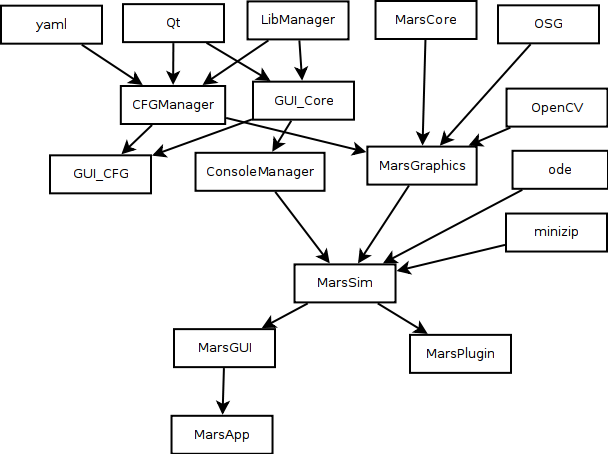
\includegraphics[width=120mm]{Diagram1.png}

\end{document}
